El trabajo colaborativo tiene un alto impacto hoy en d\'ia debido a que muchas actividades que una persona realiza son en grupo \citep{ellis1991groupware}, as\'i una actividad puede dividirse en tareas que diferentes miembros pueden hacer, esto se logra manteniendo comunicaci\'on, cooperaci\'on y colaboraci\'on entre los miembros del equipo de trabajo. La comunicaci\'on se entiende como el proceso de interacci\'on entre personas que incluye el intercambio impl\'icito o expl\'icito de informaci\'on\citep{cruz2012towards}; la coordinaci\'on es el manejo de interdependencias entre actividades realizadas por multiples actores basadas en objetos mutuos que son intercambiados entre actividades\citep{malone1994interdisciplinary}; y la cooperaci\'on ocurre cuando un grupo trabaja para lograr una misma meta  con alto grado de tareas interdependientes, compartiendo la informaci\'on disponible a trav\'es de alguna clase de espacio compartido\citep{malone1994interdisciplinary}. 

El hecho de que m\'ultiples individuos situados en diferentes escenarios de trabajo y situaciones, con diferentes responsabilidades, perspectivas y propensiones interact\'uen sean mutuamente dependientes en el conducto de su trabajo tienen implicaciones importantes en el dise\~no de sistemas computacionales dirigidos a apoyar estos esfuerzos \citep{schmidt1992taking}.

Shmidt et.al. menciona un conjunto de caracter\'isticas que se deben de tomar en cuenta para que los sistemas computacionales que estudia el CSCW sean aceptables para los usuarios \citep{schmidt1992taking}:
\begin{itemize}
\item Las unidades cooperativas son grandes o son parte de conjuntos m\'as grandes.
\item Las unidades cooperativas son, por lo general, formaciones de poca duraci\'on, emergen para manejar una situaci\'on particular y luego se disuelven.
\item La afiliaci\'on de las unidades cooperativas no son estables y normalmente no determinable. Las unidades cooperativas a veces se intersectan.
\item El patr\'on de interacci\'on en trabajos cooperativos cambia din\'amicamente con los requerimientos y restricciones de la situaci\'on.
\item El trabajo cooperativo es distribuido f\'isicamente en tiempo y espacio.
\item El trabajo cooperativo es distribuido l\'ogicamente, en t\'erminos de control, es decir, los agentes son semi-aut\'onomos en su trabajo parcial.
\item El trabajo cooperativo involucra perspectivas inconmensurables (e.g. profesiones, especialidades, funciones de trabajo, responsabilidades, etc.) as\'i como estrategias incongruentes y motivos discordantes.
\item No hay agentes omniscientes en el trabajo cooperativo en escenarios naturales.
\end{itemize}

\section{Groupware}

Existen diferentes tipos de sistemas groupware, \citep{ellis1991groupware} define dos clasificaciones: por espacio-tiempo y por tipo de aplicaci\'on. Entre el rubro espacio-tiempo se encuentran aquellos que su funcionalidad permite interacciones cara a cara o interacciones distribuidas, as\'i mismo podemos encontrar aquellos que permiten una interacci\'on en tiempo real o una interacci\'on as\'incrona. Adem\'as de groupwares s\'incronos y as\'incronos agrega un tercer rubro que combina los dos anteriores, y a\~nade el tipo de comunicaci\'on como caracter\'istica, para la interacci\'on de los usuarios usa el estado de conexi\'on de los usuarios, las interacciones distribuidas son incluidas en la categor\'ia de disponibilidad del usuario\citep{antunes2014reviewing}. Una clasificaci\'on similar es descrita por Johansen unos a\~nos atr\'as tomando en cuenta solamente las dimensiones espacio tiempo mostradas en la Figura \ref{gw:class}.

\begin{figure}[h!]
  \centering
  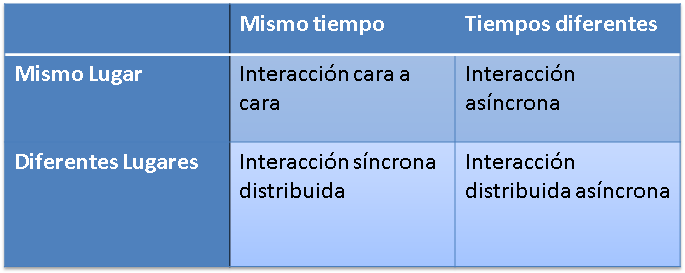
\includegraphics[scale=0.6]{dimen}
  \caption{Dimensiones de los groupware por tiempo y espacio \citep{johansen1988groupware}}
  \label{gw:class}
\end{figure}

Por otra parte cuando se toma en cuenta el tipo de aplicaci\'on para clasificar los sistemas groupware, podemos encontrar los siguientes: 
\begin{enumerate}
\item Sistemas de mensajes que soportan el intercambio as\'incrono de mensajes entre miembros de un grupo.
\item Editores multiusuario que permite a miembros de un grupo crear y editar un mismo documento al mismo tiempo, pueden ser s\'incronos o as\'incronos.
\item Sistemas para soporte de decisiones de grupo y cuartos electr\'onicos de reuniones, proveen infraestructura para la exploraci\'on de problemas no estructurados en un grupo.
\item C\'omputo para conferencias: proporciona servicios como medios de comunicaci\'on en muchas formas, hay 3 tipos: de tiempo real, teleconferencia, y de escritorio.
\item Agentes inteligentes que son programas computacionales \textit{inteligentes} encargados de tareas espec\'ificas.
\end{enumerate}

Adem\'as de la clasificaci\'on por tipo de aplicacio\'on, Ellis\citep{ellis1991groupware} propone elementos que tienen que ser tomados en cuenta para poder comparar y describir a los sistemas groupware, entre ellos se encuentran el contexto compartido que es el ambiente en el que va a correr el sistema; un grupo de ventanas que son las que se van a mostrar en diferentes pantallas del sistema y se van a compartir; un tele apuntador que es la capacidad de m\'as de un usuario de mover el apuntador al mismo tiempo; vista, es la porci\'on de contexto o ambiente que se va a mostrar en diferentes ventanas del sistema; sesi\'on que son los tipos de interacci\'on del usuario con el sistema y que ya se mencionaron antes (mismo tiempo, mismo lugar; diferente tiempo, diferente lugar, etc.) y los roles que son los tipos de usuarios que hay y los derechos y permisos que tienen con el sistema.

Shmidt \citep{schmidt1992taking} menciona varias propiedades que deben de tener los sistemas groupware que a continuaci\'on se listan:
\begin{itemize}
\item Es social; objeto, sujeto, medios, fines, motivos y necesidades, competencias e implementaciones, est\'an mediadas socialmente.
\item Integrantes mutuamente dependientes, necesitan cooperar para terminar el trabajo. Diferente a solo compartir el mismo recurso, sujeto A conf\'ia positivamente en la calidad y l\'ineas de tiempo del trabajo de sujeto B y vice versa
\item Distribuci\'on de tareas qu\'e va a hacer cada individuo, cu\'ando y d\'onde.
\item Distribuci\'on f\'isica en tiempo y espacio
\item Distribuci\'on l\'ogica, en t\'erminos de control, en el sentido de que los sistemas son semi aut\'onomos en su trabajo parcial.
\item Deben aumentar las capacidades mec\'anicas y de procesamiento de informaci\'on del individuo.
\item Deben combinar las actividades especializadas de m\'ultiples trabajadores dedicados a las diferentes herramientas especializadas.
\item Deben facilitar las aplicaciones de m\'ultiples problemas resolviendo estrategias y heur\'isticas de un problema dado.
\item Deben facilitar la aplicaci\'on de m\'ultiples perspectivas y concepciones de un problema dado para adaptarse a naturaleza m\'ultiple del ambiente de trabajo.
\item Deben apoyar la auto organizaci\'on de conjuntos cooperativos, no interrumpir trabajo cooperativo computarizando procedimientos formales.
\end{itemize}

%%%%%%%%%%%%%%%%%%%%%%%%%%%%%%%%%%%%%%%%%%%%%%%%%%%%%%%%%%%%%%%%%%%%%%%%%%

En un estudio m\'as reciente \citep{cruz2012towards} se encuentra una recopilaci\'on de los atributos pertenecientes a un groupware, entre ellas est\'an las din\'amicas de trabajo en escenarios de colaboraci\'on (comunicaci\'on, cooperaci\'on, y coordinaci\'on), dimensiones temporales y espaciales, caracter\'isticas grupales (tipos de tareas grupales, caracter\'isticas y tama\'no), categor\'ias t\'ecnicas de aplicaciones groupware (escalabilidad, software y hardware), y categor\'ias complementarias (e.g. usabilidad). En la Figura \ref{gw:stmodel} Cruz et. al. \citep{cruz2012towards} define una taxonom\'ia para groupwares organizando las categor\'ias mencionadas en la literatura general del tema orientada a entidades sociales tales como organizaciones, academias e industrias para obtener ideas sobre din\'amicas de colaboraci\'on y mejorar la calidad de interacci\'on de estas organizaciones, es por eso que esta taxonom\'ia es llamada sociot\'ecnica.

\begin{figure}[h!]
  \centering
  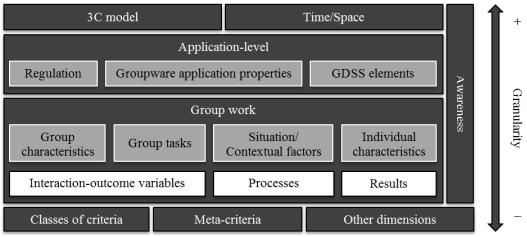
\includegraphics[scale=0.9]{socclass}
  \caption{Modelo de clasificaci\'on de groupware seg\'un Cruz \citep{cruz2012towards}}
  \label{gw:stmodel}
\end{figure}

En la Figura \ref{gw:stmodel} se observan diferentes capas que muestran las propiedades de los groupware; la primera categor\'ia se encuentra el modelo 3C, que se enfoca en la comunicaci\'on, la coordinaci\'on y la cooperaci\'on. Algunas categor\'ias de relacionadas a la coordinaci\'on en la literatura revista por Cruz \citep{cruz2012towards} son: planeaci\'on, modelos de control, relaciones entre tareas y subtareas, y manejo de la informaci\'on, ajuste mutuo, estandarizaci\'on, protocolos de coordinaci\'on, manejo temporal, recursos, o artefactos compartidos producidos durante la sucesi\'on de actividades. Entre las categor\'ias de cooperaci\'on se pueden encontrar desde producci\'on (co-autor\'ia), almacenamiento o manipulaci\'on de artefactos, hasta concurrencia, control de acceso.

Otro aspecto que toma Cruz en su modelo (Figura \ref{gw:stmodel}) es tiempo y espacio de donde se observan las siguientes subcategor\'ias: persistencia de sesi\'on, retardo en transmisi\'on de audio/video, reciprocidad y homogeneidad de canales, retardo de env\'io de mensajes, y espontaneidad de colaboraci\'on. En la categor\'ia de nivel de aplicaci\'on se identifican tipolog\'ias que clasifican a los groupware de acuerdo a su enfoque en el nivel del grupo. Como subcategor\'ia se encuentran la regulaci\'on, que son los mecanismos que permiten a los participantes organizarse en un ambiente compartido; en la literatura algunas de las dimensiones de regulaci\'on que se encuentran son: arenas(ubicaci\'on); actores(roles, lugares, y posiciones); herramientas(reguladas o no); roles(tem\'aticos o casuales); reglas(restricciones, normas o reglas de trabajo); tipos de interacci\'on; escenarios interactivos; y objetos(medios de comunicaci\'on y productos de colaboraci\'on). Otra subcategor\'ia del nivel de aplicaci\'on son las propiedades de la aplicaci\'on groupware entre las que se pueden encontrar arquitectura, cualidades funcionales y de calidad, soporte para procesos grupales, interfaz de colaboraci\'on(portales, dispositivos o espacio de trabajo f\'isico), relaciones(colecciones, listas, \'arboles y gr\'aficas), funciones de n\'ucleo, contenido(texto, ligas, gr\'aficas o flujo de datos), acciones soportadas(recibir, agregar, asociar, editar, mover, borrar, o juzgar), identificaci\'on, controles de acceso, mecanismos de alerta, componentes inteligentes, indicadores de consciencia, y plataforma, los elementos GDSS incluyen hardware, software y soporte de personas.

La siguiente capa del modelo se enfoca a los grupos, los cuales son definidos como una ``agregaci\'on social de individuos" con consciencia de su presencia, conducida por sus propias normas, y soportado por interdependencias de tareas hacia una meta en com\'un en un contexto compartido \citep{pumareja2002evolutionary}. Dentro de esta categor\'ia se encuentran las subcategor\'ias: tareas grupales, caracter\'isticas del grupo, factores de situaci\'on, y caracter\'isticas individuales.

Un groupware se puede caracterizar por 3 aspectos complementarios importantes desde la vista del usuario: una descripci\'on de los objetos y las operaciones que se pueden hacer sobre ellos y que est\'an disponibles para los usuarios, una descripci\'on de los aspectos din\'amicos del sistema (flujo de control y  de datos) y una descripci\'on de la interfaz entre el sistema y los usuarios y entre los usuarios \citep{ellis1994conceptual}. Este modelo es llamado de coordinaci\'on y describe la organizaci\'on de las actividades realizadas por los usuarios y no por el sistema. Los componentes principales de este modelo ontol\'ogico son los objetos y las operaciones. Las operaciones sobre objetos son aspectos importantes que determinan el nivel de contribuci\'on de un usuario al trabajo\citep{ellis1994conceptual}, por ej., en un sistema editor de c\'odigo colaborativo, los usuarios que realicen m\'as operaciones sobre un archivo(actualizar el archivo, crear archivo, eliminar archivo) son los que m\'as aportan al proyecto, sin embargo la desventaja de esto es que no se sabe si la operaci\'on que se hizo produjo resultados positivos, as\'i un usuario que realice varios cambios sobre un archivo puede ser se\'nal de que se equivoca mucho en su redacci\'on, otros aspectos importantes en la colaboraci\'on son la interacci\'on con miembros del grupo y el ambiente para resolver problemas, tomar decisiones, mantener la afiliaci\'on del grupo, etc.

Antunes\citep{antunes2008structuring} presenta un framework detallado para evaluar los sistemas colaborativos bajo desarrollo de acuerdo a variables dadas y niveles de desempe\~no. Considera dos dimensiones: una define el conjunto de variables de evaluaci\'on relevantes y el otro se ocupa de los niveles de desempe\'no que los usuarios evaluados. El tiempo de evaluaci\'on es inherentemente asociado con el proceso de desarrollo. Menciona una lista de m\'etodos de evaluaci\'on de groupwares son: 

\begin{itemize}
\item Evaluaci\'on heur\'istica de Groupware:(Backer et al 2002) es basado en ocho heur\'isticas groupware como una lista de caracter\'isticas que los groupware deber\'ian de tener.
\item Groupware walkthrough: (Pinelle and Gutwin 2002) un escenario es una descripci\'on de una actividad o conjunto de actividades, que incluye a los usuarios, su conocimiento, el resultado esperado y las circunstancias que los rodean.
\item Collaboration Usability Analisys (Pinelle et al. 2003): los evaluadores mapean acciones colaborativas a un conjunto de mecanismos de colaboraci\'on, o representaciones granulares de acciones colaborativas b\'asicas, que pueden estar relacionadas con elementos en la interfaz de usuario, los diagramas resultantes capturan detalles sobre componentes de tareas, una noci\'on del flujo a trav\'es de ellos y la distribuci\'on de tareas.
\item Groupware Observational User Testing (Gutwin and Greenberg 2000) los evaluadores observan como los usuarios realizan actividades particulares soportadas por un sistema en un ambiente controlado. Los evaluadores monitorean a los usuarios que tienen problemas con una tarea, o piden a los usuarios pensar en voz alta sobre lo que est\'an realizando
\item Human-Performance Model (Antunes et al. 2006): los evaluadores descomponen las interfaces en espacios de trabajo compartidos, definen escenarios cr\'iticos enfocados a acciones colaborativas para los espacios compartidos y comparan el desempe\'no del grupo en escenarios cr\'iticos para predecir tiempos de ejecuci\'on.
\item Enfoque de Manejo de conocimiento (Vizca\'ino et al. 2005): se mide si el sistema ayuda a los usuarios a detectar flujos de conocimiento y diseminar, reusar y almacenar conocimiento. El proceso de circulaci\'on de movimiento se comprende de 6 fases (creaci\'on de conocimiento, acumulaci\'on, divisi\'on, utilizaci\'on, internalizaci\'on), la evaluaci\'on se realiza contestando preguntas relacionadas a cada \'area.
\end{itemize}

El trabajo colaborativo es siempre social, en el sentido en el que el objeto y el sujeto, los fines y los medios, los motivos y necesidades est\'an mediados socialmente\citep{schmidt1992taking}, cada elemento del grupo depende, en parte, del trabajo de alg\'un otro miembro y viceversa, y cuando esto sucede, es importante que ambos elementos del grupo tengan el conocimiento de los avances del otro para poder hacer una estimaci\'on de sus propias acciones, es decir, que cada miembro est\'e conciente de lo que pasa a su alrededor para tomar decisiones adecuadas en cuanto a la actividad que tiene asignada en el grupo.

\section{Consciencia}

El ciclo de colaboraci\'on est\'a limitado por la consciencia, que es la percepci\'on del grupo acerca de lo que cada miembro desarrolla, y el conocimiento contextual que tienen sobre qu\'e est\'a pasando entre el grupo \citep{mittleman2008toward}. La consciencia en el CSCW se refiere al conocimiento que tienen los individuos sobre s\'i mismos y sobre el ambiente que los rodea, y en el caso de trabajo colaborativo, el rol que desempe\~nan en su grupo y el estado de los dem\'as integrantes, es importante que los individuos sepan lo que est\'an haciendo los dem\'as ya que pueden usar ese conocimiento para anticipar las acciones de los otros, y ayudarlos con sus tareas\citep{gutwin1996supporting}, el t\'ermino awarness(o conciencia en espa\~nol) fue introducido por primera vez por Dourish y Belloti\citep{dourish1992awareness} defini\'endolo como el entendimiento de las actividades de otros, que proporciona un contexto para tu propia actividad, este contexto es usado para asegurar que las contribuciones individuales sean relevantes a las actividades del grupo como un todo, y para evaluar las acciones individuales con respecto a los objetivos del grupo y progresos. 


En un estudio realizado por Belkadi et. al. \citep{Belkadi2013110} se listan las caracter\'isticas que debe de tener la consciencia o el conocimiento, entre ellas se encuentran el tener muchas facetas, es decir, que existen diferentes tipos de conocimiento, el conocimiento est\'a fuertemente enlazado a situaciones colaborativas ya que los colaboradores necesitan informaci\'on para llevar a cabo algunas tareas o para tomar decisiones; el conocimiento en una situaci\'on colaborativa puede incrementar los niveles de confianza entre actores lo que los alienta a compartir informaci\'on. As\'i mismo cita algunos requerimientos para permitir la consciencia, para crear un framework que apoye a la conciencia de los usuarios debe de cubrir los siguientes puntos: estar basado en frameworks te\'oricos s\'olidos, debe de modelar los elementos de una situaci\'on de manera apropiada y sus interacciones para facilitar la conciencia, debe estar basado en conceptos generales.

Adem\'as de estas caracter\'isticas proponen tres tipos consciencia: social, de las tareas y del espacio de trabajo; estas tres categor\'ias se pueden identificar con las preguntas de la Tabla \ref{aware:quest}:

\begin{center}
\begin{longtable}{|p{2cm}|p{11cm}|}
\caption{Preguntas para entender los tipos de consciencia.}
\label{aware:quest}\\
\hline
\textbf{Tipo de consciencia} & \textbf{Preguntas}\\
\hline
\endfirsthead
\multicolumn{2}{c}%
{\tablename\ \thetable\ -- \textit{Contin\'ua de p\'agina anterior}} \\
\hline
\textbf{Tipo de consciencia} & \textbf{Preguntas} \\
\hline
\endhead
\hline \multicolumn{2}{r}{\textit{Contin\'ua en siguiente p\'agina}} \\
\endfoot
\hline
\endlastfoot

	Consciencia Social & ?`Qu\'e debo de esperar de otros miembros del grupo? ?`C\'omo voy a interactuar con el grupo? ?`Qu\'e rol voy a tomar en este grupo? ?`Qu\'e roles van a tomar los dem\'as miembros del grupo? \tabularnewline \hline
	Consciencia de las Tareas & ?`Qu\'e s\'e de este tema y la estructura de la tarea? ?`Qu\'e saben los dem\'as? ?`Qu\'e se necesita para completar la tarea? ?`C\'omo ser\'an evaluados los resultados? ?`Qu\'e herramientas u objetos se necesitan para completar esta tarea? ?`Cu\'anto tiempo se necesita y cu\'anto tiempo hay disponible? \tabularnewline \hline	
	Consciencia del espacio de trabajo & ?`Qu\'e hacen los dem\'as miembros del grupo para completar la tarea? ?`D\'onde est\'an? ?`Est\'an activos en el espacio de trabajo? ?`Qu\'e har\'an? ?`Qu\'e hacen actualmente? ?`Qu\'e han hecho? ?`Qu\'e har\'an despu\'es? ?`C\'omo los puedo ayudar? \tabularnewline
	\hline

\end{longtable}
\end{center}

Cruz et. al. tambi\'en hace su propia interpretaci\'on de conciencia \citep{cruz2012towards} y la clasifica en los siguientes rubros:
\begin{itemize}
\item Consciencia espacial y atmosf\'erica
\item Consciencia de la actividad
\item Consciencia de los objetos
\item Consciencia humana
\item Consciencia presencial
\item Consciencia influencial
\item Consciencia de habilidades
\item Consciencia contextual
\end{itemize}

Antunes et. al. en su estudio \citep{antunes2014reviewing} identifica 6 tipos de conciencia, como se puede ver en la Figura entre los que se encuentran conciencia de colaboraci\'on, conciencia del contexto, conciencia social, conciencia de ubicaci\'on, conciencia de espacio de trabajo, y conciencia de la situaci\'on. Con estos tipos plantea una lista de verificaci\'on en la que se encuentran criterios de dise\~no para sistemas colaborativos.

\begin{figure}[h!]
  \centering
    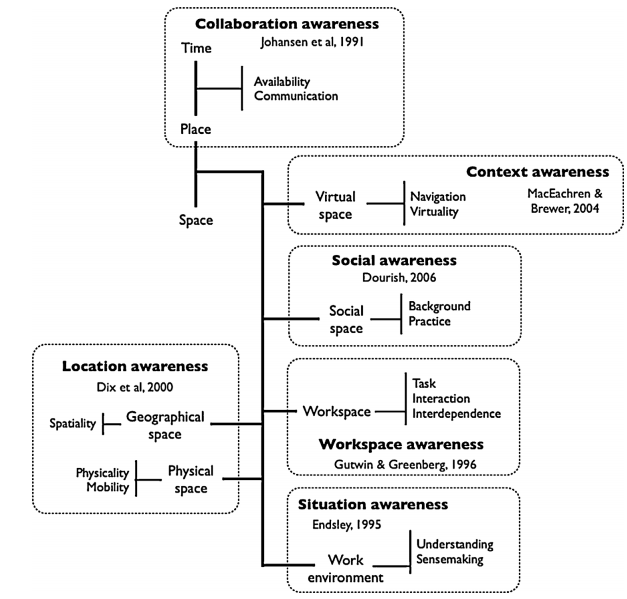
\includegraphics[scale=0.7]{antunesAwareness2012}
  \caption{Taxonom\'ia de conciencia \citep{antunes2014reviewing}}
  \label{awareness:taxonomy}
\end{figure}

La \textbf{Consciencia colaborativa} ha sido generalmente aceptado como la percepci\'on de la disponibilidad del grupo que tiene cada uno de los integrantes. Disponibilidad del grupo quiere decir el conocimiento de si las personas est\'an en el mismo lugar f\'isico, o si est\'an conectados o desconectados y los medios de comunicaci\'on que tienen disponibles para colaborar entre s\'i.

\textbf{Conciencia contextual} es el entendimiento de las actividades de los dem\'as usuarios, que proporciona un contexto para las actividades propias \citep{dourish1992awareness}, aumenta la experiencia que un individuo tiene en cualquier escenario de asistencia, el manejo de acoplamiento de actividades, la coordinaci\'on de acciones cooperativas, anticipaci\'on de actividades humanas o ambientales tanto como futuras intenciones, y la b\'usqueda de ayuda son aspectos b\'asicos de una interacci\'on que puede ser mejorada mediante la consciencia contextual \citep{aehnelt2012discussion}

La \textbf{conciencia social} apunta la importancia de entender las pr\'acticas sociales, como los roles de otros y sus actividades, o c\'omo est\'an otros miembros del grupo contribuyendo a una tarea\citep{antunes2014reviewing}.

La \textbf{conciencia de espacio de trabajo} se divide en 2 aspectos: uno se enfoca en el lugar y el otro se enfoca en el espacio, otra cosa importante a considerar es la interacci\'on del grupo con los lugares de trabajo, finalmente la noci\'on del espacio de trabajo trae consigo el nivel de interdependencia de una tarea realizada por el grupo, considerando soporte de actividades paralelas, actividades coordinadas y actividades mutuamente ajustadas.

La \textbf{conciencia situacional} est\'a caracterizada por tres niveles cognitivos: en el primero una percepci\'on global del ambiente construido por eventos, acciones, recursos y otros elementos, en el segundo nivel se le da un sentido a lo que est\'a pasando actualmente y en el tercero se construyen escenarios a futuro.

La \textbf{conciencia del lugar} puede referirse al conocimiento de los elementos de una ubicaci\'on geogr\'afica como pueden ser coordenadas, orientaci\'on, distancia, etc. O tambi\'en el conocimiento de los elementos de un espacio f\'isico, incluyendo clima, topolog\'ia f\'isica del lugar, y atributos f\'isicos.

Ya que en un sistema colaborativo se necesita estar enterado de este tipo de informaci\'on, es importante tenerla en cuenta al momento de dise\~narlos as\'i los usuarios pueden coordinarse de una mejor manera y llegar a alcanzar los objetivos que se tienen propuestos.

Por la naturaleza de los sistemas groupware las \'areas de m\'as inter\'es son la conciencia social y la conciencia del espacio de trabajo. En otra clasificaci\'on (Gutwin, C., Greenberg, S., \& Roseman, M., 1996) podemos encontrar 2 tipos de conciencia al contexto: primero conciencia general de las personas en una comunidad de trabajo, y segundo conciencia de las interacciones de otros en un espacio compartido.

Gutwin (Gutwin, Carl, Greenberg, Saul 1996) propone un marco de trabajo que considera elementos que incluyen mecanismos para recopilar informaci\'on \'util para la conciencia de la situaci\'on por parte de las personas, y que integran el conocimiento consciente del espacio de trabajo de un grupo.

\begin{center}
\begin{longtable}{|l|p{8cm}|}
\caption{Elementos de conciencia de la situaci\'on propuestos por Gutwin\citep{gutwin1996supporting}}\\
\hline
\textbf{Elementos} & \textbf{Cuestiones que responden}\\
\hline
\endfirsthead
\multicolumn{2}{c}%
{\tablename\ \thetable\ -- \textit{Contin\'ua de p\'agina anterior}} \\
\hline
\textbf{Elementos} & \textbf{Cuestiones que responden} \\
\hline
\endhead
\hline \multicolumn{2}{r}{\textit{Contin\'ua en siguiente p\'agina}} \\
\endfoot
\hline
\endlastfoot

Presencia & ?`Qui\'enes est\'an participando en la actividad?\\
Ubicaci\'on & ?`D\'onde est\'an trabajando?\\
Nivel de actividad & ?`Qu\'e tan activos son en el espacio de trabajo?\\
Acciones & ?`Cu\'ales son sus actividades y tareas actuales?\\
Intenciones & ?`Qu\'e har\'an despu\'es?, ?`D\'onde van a estar?\\
Cambios & ?`Qu\'e cambios est\'an realizando y en d\'onde?\\
Objetos & ?`Qu\'e objetos est\'an usando?\\
Extensiones & ?`Qu\'e pueden ver?, ?`Cu\'ales son sus alcances?\\
Habilidades & ?`Qu\'e pueden hacer?\\
Esfera de influencia & ?`D\'onde pueden hacer cambios?\\
Expectativas & ?`Qu\' se necesita que haga ahora?\\
\hline
\end{longtable}
\label{elem:context}
\end{center}

Los elementos de la Tabla \ref*{elem:context} se pueden clasificar en dos grupos: aquellos que se encargan de saber que est\'a pasando con otras personas, y aquellos que dan a conocer d\'onde est\'a pasando. Esta clasificaci\'on detalla el perfil individual de cada integrante y sigue las actividades de cada uno. Para facilitar la obtenci\'on de este conocimiento a los usuarios es necesario que los groupware cuenten con un mecanismo que reconozca el flujo de las actividades que se est\'an realizando. A esto se le llama conciencia contextual, que a diferencia de la conciencia que es el conocimiento que tienen los usuarios, se encarga de dotar de este conocimiento al sistema computacional para que pueda adaptarse a las actividades del equipo de trabajo.


\section{Consciencia del contexto}

Los elementos mencionados hacen referencia a la conciencia de parte del usuario del contexto que lo rodea, pero ?`es posible hacer que la conciencia del ambiente pueda ser aprendida por el propio sistema groupware? Existen groupwares capaces de reconocer aspectos contextuales que rodean a un grupo de usuarios, estos sistemas son llamados conscientes del contexto, la informaci\'on contextual m\'as com\'un en los sistemas groupware es la ubicaci\'on f\'isica del usuario. Al hablar de sistemas groupware conscientes del contexto surgen algunos asuntos importantes a tomar en cuenta, haciendo falta una categorizaci\'on formal del contexto con el que los sistemas van a modelar la situaci\'on de los usuarios, sin embargo los sistemas son desarrollados para que funcionen en \'ambitos espec\'ificos al dominio de aplicaci\'on o situaci\'on a la que se le quiere dar soluci\'on.

El conocimiento contextual describe una situaci\'on, la forma en la que se usan los elementos en un grupo de trabajo, incluyendo los eventos que son manejados por el grupo \citep{brezillon2004context}. Varios autores tienen un concepto de contexto, algunos de ellos traslapan en definici\'on con otros, y diferentes elementos son tomados en cuenta para la descripci\'on de contexto. Dey \citep{dey2001conceptual} toma varias definiciones de contexto que otros autores hab\'ian hecho antes y hace su definici\'on con un enfoque computacional, se refiere a contexto como cualquier tipo de informaci\'on que se puede usar para caracterizar la situaci\'on de entidades (se entiende por entidad una persona, lugar u objeto) que es considerada relevante para la interacci\'on entre un usuario y una aplicaci\'on incluyendo al usuario y la aplicaci\'on.

Malik \citep{malik2007future} hace referencia a varios problemas que hay en la actualidad inherentes a consciencia contextual, entre ellos est\'an la definici\'on del contexto, ya que contexto es un concepto que abarca todos los posibles par\'ametros que identifican una situaci\'on, las aplicaciones y marcos de trabajo est\'an limitados a definir los par\'ametros del contexto de su propio \'ambito. Otro problema importante es que las arquitecturas no est\'an demasiado desarrolladas aun, est\'an desarrolladas para tareas espec\'ificas, hace falta est\'andares para definir una arquitectura y herramientas, por \'ultimo otro problema que es de inter\'es para este trabajo es la interpretaci\'on del contexto y las adaptaciones del comportamiento del servicio. 

Br\'ezillon \citep{brezillon2004context} estudia tres casos de sistemas groupware conscientes al contexto y describe la forma en que apoya a la conciencia del contexto con los usuarios. SisPro es un sistema que tiene por objetivo facilitar las actividades colaborativas y procesos de aprendizaje y el desarrollo de competencias de trabajo colaborativo. SISCO tiene como tarea la preparaci\'on de reuniones,  da a conocer a los usuarios los temas de los que se est\'a hablando basados en su agenda individual. CO2DE es un software que permite unir los contextos individuales en un solo diagrama proporcionando una infraestructura de edici\'on colaborativa. 

Un caso de sistema groupware muy diferente a los anteriores es \textit{Assault Cube} \citep{montane2013context}, un juego FPS (Fisrt Shoter Person) de c\'odigo abierto que soporta las actividades colaborativas, en este varios jugadores se conectan a un servidor para llevar a cabo actividades espec\'ificas de la modalidad del juego que hayan escojido, el juego ofrece mecanismos de conciencia a los jugadores tales como un mapa de la ubicaci\'on del enemigo, un medidor de vitalidad, una pantalla de mensajes para comunicar al equipo, etc., en este sistema es crucial para los jugadores estar al tanto de los movimientos de sus compa\~neros para formmular estrategias, y tener mayor probabilidad de cumplir con los objetivos del juego.

En Figura \ref{gw:comp} se comparan los sistemas mencionados anteriormente, para realizar las comparaciones se listan algunos elementos propuestos por Gutwin \citep{gutwin1996supporting}, Montan\'e \citep{montane2013context} y Dey \citep{dey2001conceptual} estos elementos pertenecen a tres categor\'ias que son ambiente de usuario, ambiente f\'isico, y actividad; en la parte inferior de la Figura\ref{gw:comp} comparan cuatro caracter\'isticas de los groupware, el tipo de interacci\'on que apunta el tiempo en el que interact\'uan los usuarios ya sea s\'incrona, as\'incrona o mixta; la vista que ofrece el sistema, es decir, si las pantallas que muestra son compartidas por algunos usuarios o son publicas; la sesi\'on se refiere a la distribuci\'on geogr\'afica de los usuarios y el contexto que describe en que ambiente se desempe\~nan los sistemas comparados.

\begin{figure}[h!]
  \centering
    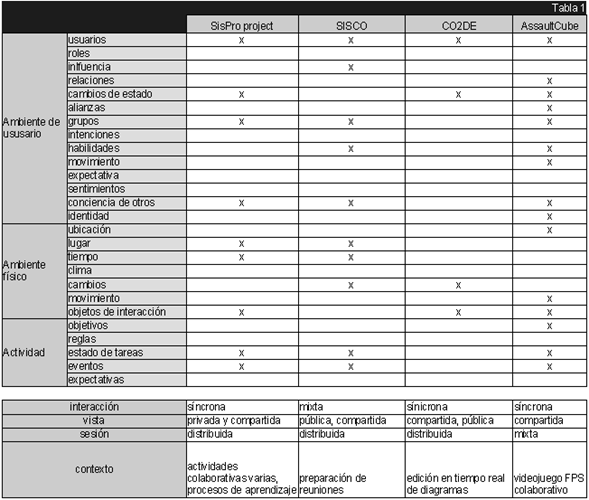
\includegraphics[scale=0.7]{groupware}
  \caption{Comparaci\'on de sistemas groupware}
  \label{gw:comp}
\end{figure}

Como se observa en la Figura \ref{gw:comp} no todos los sistemas abarcan los mismos aspectos contextuales, cada uno tiene una arquitectura singular creada para satisfacer las necesidades del entorno para el que fueron creadas, esto implica que no se pueda reutilizar el modelo de uno de ellos en los dem\'as.